\documentclass{standalone}
\usepackage{tikz}
\usepackage{ctex,siunitx}
\usepackage{tkz-euclide}
\usepackage{amsmath}
\usetikzlibrary{patterns, calc}
\usetikzlibrary {decorations.pathmorphing, decorations.pathreplacing, decorations.shapes,}
\begin{document}
\small
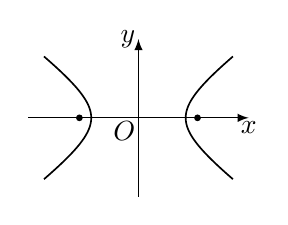
\begin{tikzpicture}[>=latex,scale=1.0,inner sep=1pt]
  \draw[thin,->](-1.4,0)--(1.4,0)node[below]{$x$};
  \draw[thin,->](0,-1)--(0,1)node[left]{$y$};
  \tkzDefPoints{0/0/O,-0.75/0/F1,0.75/0/F2}
  \draw[semithick,samples=200,domain=-60:60] plot ({0.6/cos(\x)},{0.45*tan(\x)});
  \draw[semithick,samples=200,domain=-60:60] plot ({-0.6/cos(\x)},{0.45*tan(\x)});
  \tkzDrawPoints[fill=black](F1,F2)
  \tkzLabelPoints[below left](O)
\end{tikzpicture}
\end{document}